\documentclass[utf8, 14pt, a4paper]{G7-32}% Стиль (по умолчанию будет 14pt)
\sloppy

% Настройки стиля ГОСТ 7-32
% Для начала определяем, хотим мы или нет, чтобы рисунки и таблицы нумеровались в пределах раздела, или нам нужна сквозная нумерация.
\EqInChapter % формулы будут нумероваться в пределах раздела
\TableInChapter % таблицы будут нумероваться в пределах раздела
\PicInChapter % рисунки будут нумероваться в пределах раздела

\usepackage{pscyr} 
\usepackage{float}
\usepackage{ulem}
\usepackage{xcolor}
\usepackage[textwidth=70, textsize=footnotesize]{todonotes}
\reversemarginpar

% Добавляем гипертекстовое оглавление в PDF
\usepackage[
bookmarks=true, colorlinks=true, unicode=true,
urlcolor=black,linkcolor=black, anchorcolor=black,
citecolor=black, menucolor=black, filecolor=black,
]{hyperref}

\AfterHyperrefFix

\usepackage{microtype}% полезный пакет для микротипографии, увы под xelatex мало чего умеет, но под pdflatex хорошо улучшает читаемость

% Тире могут быть невидимы в Adobe Reader
\ifInvisibleDashes
\MakeDashesBold
\fi

\usepackage{graphicx}   % Пакет для включения рисунков

% С такими оно полями оно работает по-умолчанию:
% \RequirePackage[left=20mm,right=10mm,top=20mm,bottom=20mm,headsep=0pt,includefoot]{geometry}
% Если вас тошнит от поля в 10мм --- увеличивайте до 20-ти, ну и про переплёт не забывайте:
\geometry{right=20mm}
\geometry{left=30mm}
\geometry{bottom=20mm}
\geometry{ignorefoot}% считать от нижней границы текста


% Пакет Tikz
\usepackage{tikz}
\usetikzlibrary{arrows,positioning,shadows}

% Произвольная нумерация списков.
\usepackage{enumerate}

% ячейки в несколько строчек
\usepackage{multirow}

% itemize внутри tabular
\usepackage{paralist,array}

%\setlength{\parskip}{1ex plus0.5ex minus0.5ex} % разрыв между абзацами
\setlength{\parskip}{1ex} % разрыв между абзацами
\usepackage{blindtext}

% Центрирование подписей к плавающим окружениям
%\usepackage[justification=centering]{caption}

\usepackage{newfloat}
\DeclareFloatingEnvironment[
placement={!ht},
name=Equation
]{eqndescNoIndent}
\edef\fixEqndesc{\noexpand\setlength{\noexpand\parindent}{\the\parindent}\noexpand\setlength{\noexpand\parskip}{\the\parskip}}
\newenvironment{eqndesc}[1][!ht]{%
    \begin{eqndescNoIndent}[#1]%
\fixEqndesc%
}
{\end{eqndescNoIndent}}



% % 8 Листинги

\usepackage{listings}

% Значения по умолчанию
\lstset{
  basicstyle= \footnotesize,
  breakatwhitespace=true,% разрыв строк только на whitespacce
  breaklines=true,       % переносить длинные строки
%   captionpos=b,          % подписи снизу -- вроде не надо
  inputencoding=koi8-r,
  numbers=left,          % нумерация слева
  numberstyle=\footnotesize,
  showspaces=false,      % показывать пробелы подчеркиваниями -- идиотизм 70-х годов
  showstringspaces=false,
  showtabs=false,        % и табы тоже
  stepnumber=1,
  tabsize=4,              % кому нужны табы по 8 символов?
  frame=single
}

% Стиль для псевдокода: строчки обычно короткие, поэтому размер шрифта побольше
\lstdefinestyle{pseudocode}{
  basicstyle=\small,
  keywordstyle=\color{black}\bfseries\underbar,
  language=Pseudocode,
  numberstyle=\footnotesize,
  commentstyle=\footnotesize\it
}

% Стиль для обычного кода: маленький шрифт
\lstdefinestyle{realcode}{
  basicstyle=\scriptsize,
  numberstyle=\footnotesize
}

% Стиль для коротких кусков обычного кода: средний шрифт
\lstdefinestyle{simplecode}{
  basicstyle=\footnotesize,
  numberstyle=\footnotesize
}

% Стиль для BNF
\lstdefinestyle{grammar}{
  basicstyle=\footnotesize,
  numberstyle=\footnotesize,
  stringstyle=\bfseries\ttfamily,
  language=BNF
}

% Определим свой язык для написания псевдокодов на основе Python
\lstdefinelanguage[]{Pseudocode}[]{Python}{
  morekeywords={each,empty,wait,do},% ключевые слова добавлять сюда
  morecomment=[s]{\{}{\}},% комменты {а-ля Pascal} смотрятся нагляднее
  literate=% а сюда добавлять операторы, которые хотите отображать как мат. символы
    {->}{\ensuremath{$\rightarrow$}~}2%
    {<-}{\ensuremath{$\leftarrow$}~}2%
    {:=}{\ensuremath{$\leftarrow$}~}2%
    {<--}{\ensuremath{$\Longleftarrow$}~}2%
}[keywords,comments]

% Свой язык для задания грамматик в BNF
\lstdefinelanguage[]{BNF}[]{}{
  morekeywords={},
  morecomment=[s]{@}{@},
  morestring=[b]",%
  literate=%
    {->}{\ensuremath{$\rightarrow$}~}2%
    {*}{\ensuremath{$^*$}~}2%
    {+}{\ensuremath{$^+$}~}2%
    {|}{\ensuremath{$|$}~}2%
}[keywords,comments,strings]

% Подписи к листингам на русском языке.
\renewcommand\lstlistingname{Листинг}
\renewcommand\lstlistlistingname{Листинги}

% Любимые команды
\newcommand{\Code}[1]{\textbf{#1}}

\usepackage[russian, english]{babel}
\usepackage{cite}

\begin{document}

%%%%%%%%%%%%%%%%%%%%%%%%%%%%%%%%%%%%%%%%%%
% НАЧАЛО ТЕКСТА

%	Тут можно начинать писать текст.
\section*{Введение}
\addcontentsline{toc}{chapter}{Введение}
В процессе автоматизации производства, при расчете расписания работы сотрудников либо прогнозировании сроков выполнения заказов, существует необходимость привязки абстрактных расчетов, базирующихся на времени выполнения операций, к конкретно заданному календарю производственной площадки, который учитывает выходные дни, праздничные и шаблонные смены занятых сотрудников. Данный шаг позволяет оценить применимость составленного расписания в данных условиях и оценить реальные сроки выполнения заказа.
\todo[inline]{почему Go}
\newpage
\tableofcontents
\chapter{Обзорная часть}\todo{rename?}
\todo[inline]{Написать переход}
% \section{Индустрия 4.0}
Индустрия 4.0 -- прогнозируемое массовое внедрение киберфизических систем в промышленность и повседневный быт человека, что приведет к автоматизации бизнес-процессов предприятий.
Также внедрение киберфизических систем в быт повысит качество жизни людей путем автоматизации многих повседневных циклических действий.
Под киберфизической системой (CPS~--~cyber-physical system) подразумевается взаимодействие цифровых, аналоговых, физических и человеческих компонентов, разработанных для функционирования посредством интегрированной физики и логики или другими словами: киберфизические системы -- это интеллектуальные системы, которые состоят из тесно взаимосвязанных сетей физических и вычислительных компонентов\cite{nist}.\\
\indent Появилось понятие индустрии 4.0 во время ганноверской выставки 2011 года как обозначение стратегического плана развития и поддержания конкурентоспособности немецкой экономики, предусматривающий совершение прорыва в области информационных технологий для промышленности.
Также считается, что данное направление знаменует собой четвертую промышленную революцию\cite{industry}.\\
\indent Как можно понять из названия, четвертая промышленная революция в первую очередь ориентирована на промышленность.
Рассматривая данную область, процесс внедрения киберфизической системы разделяется на внедрение физической части (датчики, микроконтроллеры, и так далее...) и вычислительную -- систему планирования производства.\\
\indent Система планирования производства (СПП) обеспечивает расчет объемно-календарного и оперативного планов, автоматизированный подбор поставщиков, автоматизированный перерасчет планов по фактическим результатам деятельности, направленный на минимизацию временных и финансовых потерь.\\
\indent Объемно-календарный план -- задание для каждой производственной площадки на заданный интервал времени, представляющее собой план-график, на котором каждому интервалу соответствует номенклатура и объем подлежащих к производству изделий\cite{niokr}.\\
\indent Оперативный план -- план, согласно которому выполняется сопоставление каждой операции для каждой единицы продукции к временным интервалам, конкретному работнику и конкретным производственным средствам\cite{niokr}.\\
% \indent С некоторыми оговорками можно сказать, что оперативный план является более подробной версией объемно-календарного плана, которая, в силу ограничений со стороны вычислительной сложности расчета, составляется на срок в порядок меньший, чем для объемно-календарного плана.
% \to\do[inline]{схема и сравнение планов}

\section{Обзор существующих решений}
\indent Сегодня, чтобы сохранять конкурентоспособность, предприятиям необходимо развивать и внедрять системы управления и планирования производственных процессов. 
Актуальным направлением, ориентированным на решение этой задачи, является разработка СПП, которая должна обеспечивать решение следующих задач: исполнения планов производства и целевых показателей, оптимизации операционной деятельности, снижения затрат и повышения эффективности производства.\\
\indent Производственное планирование — это систематический, структурированный, направленный на достижение поставленной задачи процесс планирования промышленного предприятия, состоящий из отдельных, иерархически распределенных этапов, осуществляемый с помощью специальных методов и инструментов, начиная с момента появления замысла и заканчивая запуском производства \cite{mulBook}.
Производственное планирование может также включать в себя корректирующие мероприятия в процессе эксплуатации. Планирование промышленного предприятия может основываться на различных целях и задачах, охватывать самые разные проектные ситуации.\\
\indent В процессе планирования используется ряд инструментов и программных компонент, которые поддерживают реализацию метода планирования \cite{lodonBook}.
Говоря в общем, это программные средства (прикладные программы), которые применяются пользователями на персональных компьютерах в различных фазах планирования жизненного цикла промышленного предприятия.
К основным инструментам планирования относятся: APS/SCM; САР; АСУП. 
Ниже даны подробные описания данных типов инструментов \cite{oliriBook}.\\
\indent APS/SCM (системы синхронного планирования, системы управления логической цепочкой) поддерживают расчеты, эксплуатацию и оптимизацию логистических цепочек. 
Особые свойства логистической цепочки получаются благодаря взаимодействию участников. 
Важная роль отводится структуре логистических цепочек, соответствующих рынку, а также координации и интеграции всех индивидуальных действий.\\
\indent САР (система автоматизированного регулирования) характеризует область компьютеризованного планирования работы. 
При этом используется система электронной обработки данных для создания рабочего графика, выбора эксплуатационных средств, создания указаний по изготовлению и монтажу, а также программирования для ЧПУ.\\
\indent АСУП (САМ — автоматическая система управления производством) включает в себя компьютерное техническое управление и контроль над производственными линиями и эксплуатационными средствами при проведении производства, т.е. прямое управление обрабатывающими и перерабатывающими машинами, устройствами манипуляции, транспортировки, перегрузки и хранения, а кратко — техническое управление всеми устройствами потоковых систем \cite{gibBook}.\\
\indent Наиболее распространенными программными продуктами, предназначенными для планирования производственных процессов являются «1С:Предприятие» и «SAP R/3»: первый является наиболее распространенным на российском рынке, второй, в свою очередь, широко используется за рубежом. 
На примере этих, зарекомендовавших себя с положительной стороны продуктов проведем анализ системных компонент и сравним их место в архитектуре систем.

\subsection{«1С: Предприятие 8.0»}

\indent Комплекс программ «1С: Предприятие 8.0» состоит из технологической платформы и прикладных компонентов, которые создаются на её основе и предназначены для автоматизации деятельности предприятий. 
Технологическая платформа не является готовым программным продуктом, предназначенным для внедрения на предприятие, вместо нее обычно применяют несколько компонентов, разработанных на её базе.
Данное решение делает возможным автоматизировать различные виды деятельности, применяя единую основную технологическую платформу.\\
\indent Система «1С: Предприятие 8.0» использует следующие основные компоненты:

\begin{itemize}
	\item «Управление торговлей»;
	\item «Управление персоналом»;
	\item «Управление производственным предприятием»;
	\item «Управление складом»;
	\item «Управленческий учет и расчет себестоимости».
\end{itemize}

\indent Наиболее интересными для рассмотрения являются компоненты «Управление персоналом» и «Управление производственным предприятием», поскольку их реализация является ключевой с точки зрения планирования деятельности предприятия и не имеет сегодня строгой математической формализации.\\
\indent Компонент «1С: Предприятие 8.0. Управление персоналом» позволяет эффективно управлять кадровыми процессами в следующих областях: планирование потребностей в персонале; обеспечение организации новыми кадрами; эффективное планирование занятости персонала; кадровый учет и анализ персонала; управление персоналом.\\
\indent Компонент «Управление производственным предприятием» предназначена для автоматизации процессов управления и учета производственном предприятии.
Это позволяет создать единую информационную систему для управления различными сторонами деятельности предприятия.\\
\indent В платформе «1С: Предприятие 8.0» заложен ряд подходов, которые формируют основную концепцию разработки типовых компонентов. 
Эти подходы предназначены для максимального сближения технологических возможностей с бизнес-процессами разработки и интеграции прикладных решений.
Важными моментами, которые следует отметить, являются: изоляция разработчика от технологических деталей, алгоритмическое программирование конкретной бизнес-логики приложения, использование собственной модели базы данных и гибкость прикладных решений без их доработки.\\
\indent Механизм обмена данными, используемый в технологической платформе «1С: Предприятие 8.0», позволяет создавать территориально распределенные информационные системы на основе баз данных «1С: Предприятия 8.0», и использовать другие информационных систем, не относящиеся к «1С: Предприятии 8.0».
Например, можно организовать работу главного офиса, филиалов и складов предприятия в одной базе данных, или обеспечить взаимодействие базы данных «1С: Предприятия 8.0» с существующей базой данных «Oracle».\\
\indent Технологическая платформа «1С: Предприятие 8.0» предоставляет средства разработки, с помощью которых создаются новые или модифицируют существующие прикладные решения.
Этот инструмент разработки называется «конфигуратор».
Благодаря тому, что он поставляется со стандартным пакетом «1С: Предприятия 8.0», то пользователь может свободно разработать или модифицировать прикладное решение (адаптировать его под себя), возможно, с привлечением сторонних специалистов.\\
\indent Среди преимуществ данной системы можно выделить:

\begin{itemize}
	\item открытость системы;
	\item регулярные программные обновления;
	\item широкие функциональные возможности системы.
\end{itemize}


\indent Однако необходимо отметить, что подходы «1С: Предприятия» ориентированы на решение проблем автоматизации бухгалтерского и организационного управления предприятием.
Использование проблемно-ориентированных объектов позволяет разработчику решать задачи складского, бухгалтерского, управленческого учета, расчетам заработной платы, анализа данных и управлению бизнес-процессами.
Однако области экономического и бухгалтерское учета характеризуются высокой степенью математического формализации и их реализация происходит с относительно малыми трудозатратами, тогда как компоненты планирования и производственного расписания сегодня являются актуальными направлением для исследований и прикладной разработки.

\subsection{«SAP R/3»}

\indent Система «SAP R/3» предоставляет собой набор разноплановых инструментов, направленных на повышение эффективности производственного процесса, увеличение экономической стабильности, автоматизацию процессов планирования.
Она дает возможность интегрировать инновационные подходы централизованного планирования и управления, и повысить качество управления на разных организационных уровнях предприятий.\\
\indent «SAP R/3» использует модульную архитектуру, где каждый отдельный модуль предназначен, для решения специализированной задачи процесса предприятия, взаимодействие между ними происходит в режиме реального времени. 
Наибольший интерес для рассмотрения представляют компоненты, не имеющие прямого отношение к бухгалтерской и экономической деятельности предприятия - модуль PP; модуль HR; модуль BC.\\
\indent Модуль PP (планирование производства) дает возможность организовать управление и планирование производства предприятия.
Модуль PP реализует следующие функции: формирование спецификаций, создание технологических карт, управление производственными площадками, планирование сбыта, планирование потребности в материалах, управление производственными заказами, планирование затрат на изготовление изделие, учет затрат производственных процессов, планирование производственной деятельности, управление серийным производством, планирование автоматизированного производства.\\
\indent Модуль HR (управление персоналом) решает задачи планирования и управления работой персонала. 
Ключевые элементы: администрирование персонала, расчет данных для вычисления заработной платы, сбор и анализ данных о рабочем времени, учет командировочных расходов, создание информационной модели внутренней структуры компании.\\
\indent Модуль BC (базовый модуль) предназначен для интеграции в систему «SAP R/3» всех отдельных прикладных модулей и обеспечивает независимость от аппаратной платформы. 
Модуль BC позволяет организовать работу c многоуровневой распределенной архитектуре клиент-сервер. 
Система «SAP R/3» работает на серверах UNIX, AS/400, Windows NT, S/390 и с различными СУБД (Informix, Oracle, Microsoft SQL Server, DB2). \cite{mazBook}.\\
\indent На данный момент система «SAP R/3» является наиболее распространенной системой управления предприятием. 
Благодаря тому, что она является модульной системой, ее можно настроить в соответствии с конкретными потребностями отдельного предприятия. 
Степень технического уровня системы определяется возможностью ее перенастройки без необходимости переписывать программный код. 
Эта опция «SAP R/3» также позволяет занимать ведущее место в мире в системе управления.\\
\indent С помощью инструментов управления, включенных в систему «SAP R/3», можно реализовывать задачи мониторинга и анализа, без дополнительного программирования, следующие способы:

\begin{itemize}
	\item мониторинг БД; 
	\item мониторинг операционной системы сервера; 
	\item мониторинг коммуникаций;
	\item мониторинг и управление сервером приложений:
	\begin{itemize}
		\item формирование и запуск новой конфигурация ядра R/3; 
		\item снятие и редактирование текущей конфигурации ядра R/3; 
		\item формирование временного графика в зависимости от нагрузки (например, в ночное время можно увеличивать количество процессов, отвечающих за фоновые задания); 
		\item управление системой архивирования; 
		\item управление текущими пользователями, процессами. 
	\end{itemize}
\end{itemize}

\indent Многоуровневая клиент-серверная архитектура позволяет разделять задачи управления данными, ориентированные на пользователя.
В версии 3.0 системы «SAP R/3» SAP AG были расширены возможности решения для взаимодействия с другими приложениями и расширены возможности распределения операций «SAP R/3» в масштабируемой компьютерной структуре. 
Технология внедрения «SAP R/3» основана на многоуровневой архитектуре с использованием программного обеспечения среднего уровня. 
Между тем, промежуточное ПО отделяет пользовательские приложения от аппаратного и программного обеспечения, с другой стороны, решает проблему взаимодействия программных приложений и аппаратного обеспечения. 
В «SAP R/3» SAP Basis функционирует как промежуточное программное обеспечение \cite{mazBook}.\\
\indent Основные данные — это информация, которая хранится в базе данных, достаточно долгий промежуток времени. 
К ним относятся такие данные как: информация о кредиторах, поставщиках, материалах и счетах. 
Основные данные создаются централизованно и доступны для всех приложений. 
Например, они включают данные клиента, которые используются в заявках, поставках, выставления счетов и платежей. 
Основные данные клиента могут быть присвоены следующим организационным единицам: балансовая единица, сбытовая организация, канал сбыта, сектор.\\
\indent Основная запись материала является центральным объектом данных системы «SAP R/3». 
Она включает в себя: сырье; оборудование; расходные материалы; полуфабрикаты; продукты; вспомогательное производственное оборудование и инструменты. 
Она является главным источником данных предприятия и используется всеми компонентами логистической системы SAP. 
Благодаря объединению всех материалов в единый объект базы данных устраняются проблемы избыточности данных. 
Сохранённые данные могут использоваться во всех областях, такими как закупки, контроль запасов, планирование потребностей в материалах, проверка счетов.\\
\indent Данные, хранящиеся в основной записи материала необходимы логистическому модулю системы для решения следующих задач: обработки запасов на поставку; обновления движения материалов и инвентаризационной обработки; проводки счетов; обработки клиентских заказов; планирования потребностей и календарного планирования. 
Структурная логика поставщика и клиента также применяется к основной записи материала. 
При оформлении заказа для клиентов необходимо учитывать: согласование о перевозке, условия доставки, оплаты и т.д. 
Данные, необходимые для таких операций, дублируются из основной записи делового партнера, чтобы исключить необходимость повторного ввода информации о каждой транзакции. 
В основной записи материала могут одновременно храниться данные, обработанные во время ввода заказа, например, цена за единицу цены товара, запасы на другом складе и т.д. 
Этот принцип полезен для обработки данных в каждой основной записи, связанной с выполнением операции.\\
\indent Для каждой транзакции необходимо присваивать соответствующую организационную единицу. 
Присвоение структуры предприятия генерируется в дополнение к данным, доступным по данным клиента и по данным материала. 
Поэтому документ, созданный при помощи транзакции, содержит все основные данные из организационных единиц \cite{gehBook}.\\
\indent Среди достоинств данной системы можно выделить:

\begin{itemize}
	\item прозрачность деятельность предприятия;
	\item повышение оборотов товарно-материальных запасов;
	\item сокращение персонала управления;
	\item единые стандарты управления.
\end{itemize}

\indent К недостаткам относятся:

\begin{itemize}
	\item требуется высокий уровень подготовки персонала;
	\item сложность интеграции;
	\item большие финансовые вложения.
\end{itemize}

 % Начинается с новой страницы, так как содержит Главу (Chapter).
\chapter{Разработка компонент системы планирования производства}
\section{Архитектура системы планирования производства}
\indent Система планирования производства представляет из себя набор программных модулей, как представлено на рисунке \ref{fig:archSPP}.

\begin{figure}[ht]
	\centering
	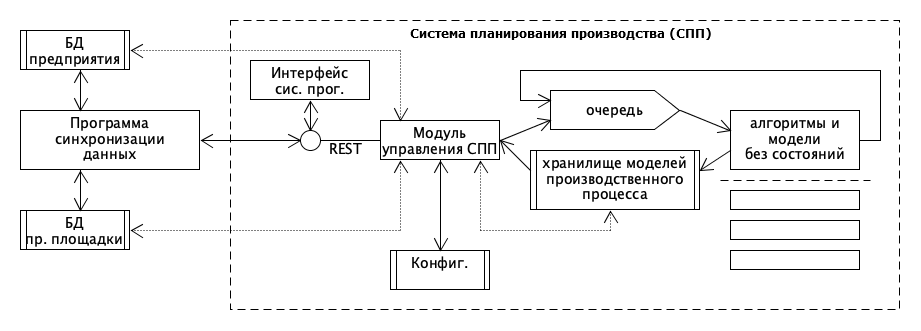
\includegraphics[width=\linewidth]{pics/archSPP.png}
	\caption{Схема системы планирования производства \cite{niorkpz}}
	\label{fig:archSPP}
\end{figure}

\indent Так как для выбора оптимального плана человеку требуется несколько планов, собственно из которых и нужно будет выбрать нужный, система производит запуск множества параллельных расчетов, каждый из которых отличается конфигурацией смен либо количества доступных ресурсов.
За запуск и синхронизацию отвечает ``Модуль управления СПП'' (\ref{fig:archSPP}), который создает очередь расчетов на запуск.
Затем пул потоков извлекает их в порядке очереди и начинает работу ядра имитационного моделирования ("Алгоритмы и модели без состояний", рисунок \ref{fig:archSPP}).
После окончания работы полученный результат передается обратно в модуль управления для возврата пользователю посредством RESTful API(REST~-~архитектурный стиль взаимодействия компонентов распределённого приложения в сети).
Пользователь, зная с какими параметрами запускался полученный расчет, может поменять конфигурацию и отправить на повторное вычисление, что будет сохранено в базе данных предприятия и запустит весь цикл заново.
\section{Подсистема имитационного моделирования}
\indent Подсистема имитационного моделирования - модуль, производящий моделирование производственных процессов для для получения приблизительной оценки времени выполнения набора операций (например карты технологического процесса).\\
\indent Карта технологического процесса - документ, предназначенный для операционного описания технологического процесса изготовления или ремонта изделия (составных частей изделия) в технологической последовательности по всем операциям одного вида формообразования, обработки, сборки или ремонта с указанием переходов, технологических режимов и данных о средствах технологического оснащения, материальных и трудовых затратах.\\
\indent Для определения оценки времени модуль рассматривает карту технологического процесса как систему уравнений, в которой неизвестными являются времена начала выполнения операций.
Каждое уравнение предстает в виде $x_n = x_{n-1} + dur$, а система в целом:
\todo{система уравнений и технологическая карта}
\begin{equation}
	x_n = x_{n-1} + dur
\end{equation}

\indent В начале работы система выберет одно из уравнений (в зависимости от накладываемых моделью ресурса, о которой пойдет речь в следующем разделе, ограничений), которое может быть рассчитано, то есть которое может начинаться с логического нуля и произведет подсчет времени, когда закончится выполнение данной операции.
Затем по тому же принципу будет выбрано следующее уравнение и так далее пока есть неразрешенные переменные.
Когда они закончатся система завершит свое выполнение, передав результирующее значение и необходимые данные другому модулю, который произведет отображение полученного подсистемой имитационного моделирования числа в физическое, о чем речь пойдет ниже.

\todo[inline]{система уравнений}
\todo[inline]{схема и описание}

\section{Модель ресурса сборочной линии}
\indent В процессе создания оперативного плана, для получения корректной оценки времени выполнения операции или набора операций СПП необходимо ввести систему ограничений, которая будет отражать как ресурс, участвующий в операции может влиять на её время выполнения.
Это привело к созданию модели ресурсов накладывающей ограничения на выбор операции для расчета ядром имитационного моделирования.
Под ресурсом подразумевается любое устройство,деталь,инструмент или средство,за исключением сырьевого материала и промежуточного продукта, находящиеся в распоряжении предприятия для производства товаров и услуг.
В соответствии с данным определением к ресурсам относятся в том числе и человеческие ресурсы, которые в данной системе не рассматриваются с точки зрения поведения или других аспектов человеческой жизни, а лишь с точки зрения возможности выполнить конкретную задачу.
Также необходимо обозначить, что в данном разделе под моделью ресурса будет пониматься упрощенная модель реального ресурса, отражающая его основные (в рамках выполняемых операций) характеристики.\\
\indent Каждая модель ресурса представляет из себя структуру данных, которая должна реализовывать три метода:
\begin{itemize}
	\item метод привязки операции к модели ресурса;
	\item метод, осуществляющий проверку возможности выполнения данной операции моделью ресурса;
	\item метод, осуществляющий логику работы и в котором происходит изменение состояния данной модели.
\end{itemize}

\indent Под привязкой операции к модели подразумевается добавление операции в очередь на выполнение и, если это первая привязанная для данного продукта операция, то добавление продукта в очередь на распределение. Привязка осуществляется в начале работы системы, что позволяет ресурсам манипулировать ядром имитационного моделирования разрешая или запрещая выбирать привязанные к ним операции для расчета, что может повлечь за собой изменение последовательности выполнения операций и, соответственно, расчетного времени выполнения карты технологического процесса.\\
\indent Проверка производится во время работы системы и именно здесь происходит отбор операций в соответствии с внутренним состоянием модели.\\
\indent Логика осуществляется при выборке операции ядром и для каждой вызывается два раза: чтобы отметить состояние модели в начале и в конце расчета операции (см. \ref{fig:assemblyResSchema}).

\begin{figure}[h]
	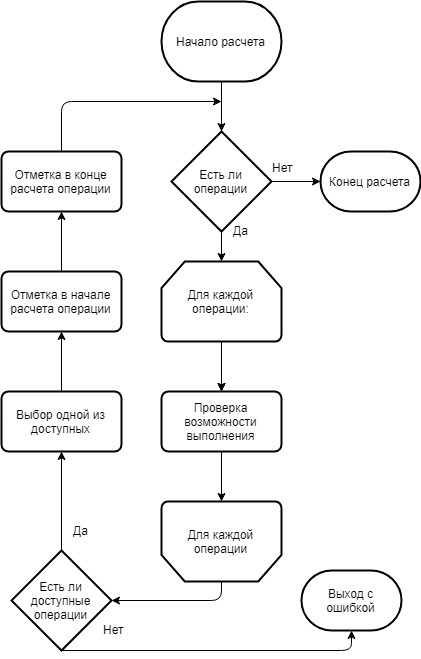
\includegraphics[scale=0.7]{pics/assemblyResSchema.png}
	\caption{Схема работы ядра моделирования с ресурсами в процессе расчета оперативного плана}
	\label{fig:assemblyResSchema}
	\centering
\end{figure}

\indent СПП имеет несколько видов ресурсов, одним из которых является модель ресурса сборочной линии, который описывает несколько однотипных, то есть с одинаковым числом рабочих постов, физических сборочных линий.
Сборочная линия - это способ перемещения заготовки от одного рабочего поста к другому; на каждом посту выполняются закрепленные за ним операции.
Под постами понимаются заготовко-места, оснащенные соответствующим технологическим оборудованием и предназначенными для технического воздействия на заготовку для осуществления фиксированного перечня операций.
Объединение нескольких сборочных линий в одну обуславливается упрощением как взаимодействия с ядром имитационного моделирования так и упрощением управления моделью потому как в любом случае (даже когда все линии будут различны по количеству постов) количество линий в модели будет всегда меньше либо равно количеству физических сборочных линии, а также возможностью инкапсуляции реализации распределения заготовок и связанных с ними операций по сборочным линиям внутри модели.

\begin{figure}[h]
	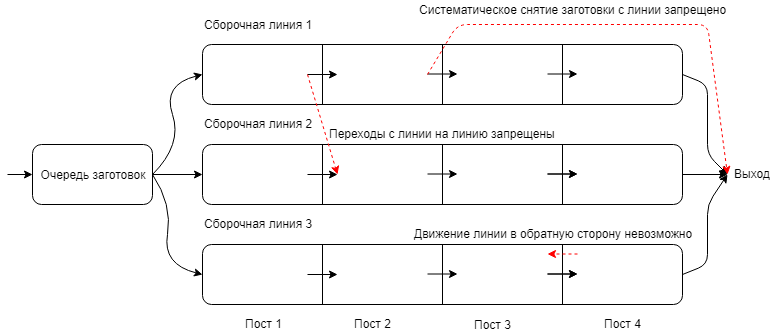
\includegraphics[width=\linewidth]{pics/assemblyMain.png}
	\caption{Схема модели ресурса с вариантами перемещения заготовки внутри}
	\label{fig:assemblyMain}
	% \centering
\end{figure}

\indent Главным предназначением данной модели является ограничение перемещения продукции внутри ресурса (см. \ref{fig:assemblyMain}), и моделирование работы физического сборочного конвейера.
С одной стороны ограничивается перемещение между сборочными линиями: к какой продукт был привязан, на той он и останется до окончания выполнения всех операций, относящихся к данному продукту и привязаны к постам данной сборочной линии.
С другой - ограничивается перемещение продукции между рабочими постами: продукт должен двигаться последовательно с поста на пост (см. \ref{fig:assemblyMain}).\\
\indent Одной из ключевых особенностей практически любой сборочной линии является синхронизация передвижения продукции между постами. 
Это означает что такт производства (время,в течение,которого заготовка пребывает на посту) будет равен максимальной временной отметке среди всех постов или другими словами: каждая заготовка сможет сменить пост только после того, как все остальные заготовки будут готовы к смене своих постов.\\
\indent Для реализации необходимого функционала, были введены структуры, описывающие линии, посты, очередь продукции, и проекцию привязки операций к постам линий.
Каждая из линий модели сборочной линии характеризуется временем начала текущего рабочего такта сборочной линии, максимальным временем рабочего такта и набором рабочих постов, каждый из которых описывается состоянием (выполняются работы, простаивает, отсутствует продукция на посту), временной меткой данного поста и продукцией, которая на данный момент находится на нем.
Максимальное время отражает какое время работал пост с начала работы системы.
Так как карта технологического процесса позволяет, при возможности, производить параллельные операции над заготовкой, то необходимо знать, с какого времени был начат такт, для чего и вводится время начала работы поста.
Время начала текущего рабочего такта показывает время с которого началась работа на текущем посту над текущей заготовкой и для всех постов она равна (из-за синхронизации постов).\\
\indent Проекция привязки операций к постам линий - структура данных необходимая для динамической привязки операций.
Так как во время привязки операции система не может оценить время выполнения продукции и, следовательно, распределив продукты до начала работы может сложиться ситуация, когда одна из линий будет работать намного дольше или наоборот по сравнению с другими линиями, что может привести к простою производству.
Следовательно необходимо, не привязывая операцию к определенной линии, обозначить к какому посту относится операция (см. \ref{fig:bind}).
Для этого и была создана данная структура, содержащая то же количество постов что и остальные линии, но не описывающая какую либо физическую сборочную линию, а являющуюся по сути проекцией всех остальных.
Внутри каждого поста данной проекции находится хэш-таблица (структура данных, позволяющая хранить пары (ключ, значение) и выполнять три операции: операцию добавления новой пары, операцию поиска и операцию удаления пары по ключу), в которой ключом является конкретная единица продукции, характеризуемая типом продукции (названием) и серийным номером, а значением - список операций, которые необходимо выполнить над данным продуктом на данном посту.

\begin{figure}[h]
	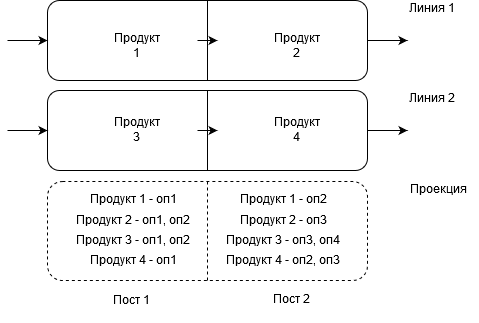
\includegraphics[width=\linewidth]{pics/assemblyBind.png}
	\caption{Схема сборочной линии с проекцией привязки операций к постам}
	\label{fig:bind}
\end{figure}

\indent Во время выполнения система, для определения возможности выполнения операции опрашивает все линии с целью определения возможности выполнения данной операции и местонахождения продукта:

\begin{itemize}
	\item при отсутствии продукта на всех линиях:
		\begin{enumerate}
			\item[1)] инициируется проверка всех линий на возможность загрузки первого поста (то есть пуст ли он);
			\item[2)] из получившегося списка линий (если количество больше нуля, иначе переход к \ref{itm:point4}) выбирается линия, временная отметка которой является наименьшей среди всех доступных линий;
			\item[3)] возвращается разрешение на выполнение данной операции и временная метка, выбранная на предыдущем шаге;
			\item[\mylabel{itm:point4}{4})] иначе (количество линий равно нулю) возвращается запрет на выполнение данной операции на текущей итерации.
		\end{enumerate}
	\item если продукт находится на какой-либо линии, то производится опрос проекции:
		\begin{enumerate}
			\item при нахождении нужной операции на посту, на котором находится в данный момент продукт, возвращается разрешение на выполнение и временная метка, с которой может производиться данная операция;
			\item иначе возвращается запрет выполнения.
		\end{enumerate}
\end{itemize}

\indent Ядро имитационного моделирования последовательно переберет все доступные на данной итерации и выберет одну из тех, что получили разрешение от всех моделей на выполнение.
Если таковых не будет, то система известит о невозможности дальнейшей работы вследствие логической ошибки при задании входных данных.
В ином случае произойдет вызов метода для того, чтобы отметить состояние модели в начале выполнения операции.
При этом если продукт не был загружен на линию, то произойдет загрузка продукта на линию с минимальной временной отметкой, иначе произойдет проверка на возможность сдвига линии.\\
\indent Во второй раз метод будет вызван для того, чтобы отметить окончание операции, что означает что данная операция будет удалена из проекции, временная метка поста будет изменена с учетом длительности операции, и, если операций на данном посту для данного продукта не осталось, то состояние поста изменится на 'готов к сдвигу линии' и будет совершена проверка возможности сдвига линии.

\begin{figure}[h]
	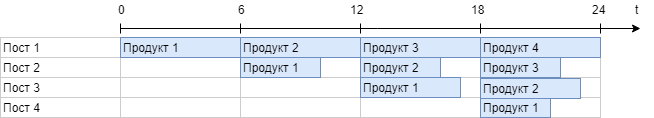
\includegraphics[width=\linewidth]{pics/assemblyDiagram.png}
	\caption{Диаграмма, изображающая сдвиг линии}
	\label{fig:lineDiagram}
\end{figure}

\indent Сдвиг линии - процесс, при котором все посты на сборочной линии передают свою заготовку на следующий пост и принимают заготовку с предыдущего.
Данный процесс единовременен для всех постов, не может быть разделен или проигнорирован каким-либо постом и выполняется после получения от всех постов сигнала о готовности к сдвигу.
При этом происходит синхронизация постов, то есть все посты, и, соответственно вся линия, получают одну временную отметку - сумма предыдущей отметки начала рабочего такта и длительности текущего рабочего такта линии.
С этой отметки начинается отсчет следующего такта (см. \ref{fig:lineDiagram}).

\begin{figure}[h]
	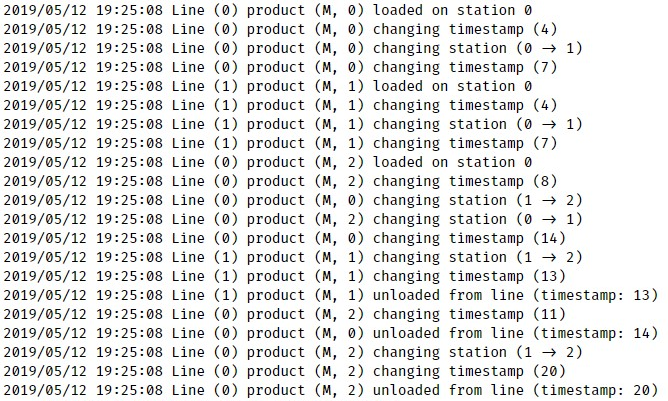
\includegraphics[width=\linewidth]{pics/assemblyResult.png}
	\caption{Лог с результатами работы модели ресурса сборочной линии}
	\label{fig:lineResult}
\end{figure}

\indent Для наглядного представления процессов происходящих в данной модели, на каждой итерации работы, создается несколько записей в лог для отслеживания состояния модели в данный момент и по которым можно отследить некорректное поведение либо просто узнать причины, по которым ядро имитационного моделирования отработало именно в такой последовательности (естественно при условии работы с моделью ресурса сборочной линии).
На рисунке \ref{fig:lineResult} видно, что модель ресурса охватывает две линии (0 и 1) физических конвейеров и работает с тремя продуктами типа 'М' (0, 1 и 2).
Также в данном логе видны все передвижения продуктов между постами (station) и все изменения временных меток и результирующие метки при выгрузке с последних постов.\\
\indent По завершении основной разработки было произведено ручное тестирование (просмотром логов в поисках ошибок работы, рисунок \ref{fig:lineResult}), так и автоматизированное с написанием автоматизированных как модульных (для проверки самой модели) так и нескольких интеграционных тестов для проверки работы с ядром имитационного моделирования и другими моделями ресурсов, которые показали правильную работу во всех рассмотренных случаях.

\section{Модуль отображения логического времени на физическое}
\indent Так как расчет выполнения операции (как и всей карты технологического процесса) ядром имитационного моделирования производится в логическом времени,то есть во времени отсчитываемом от нуля, существует необходимость в отображении (соответствие между элементами двух множеств) логического времени на физическое, которое используется в повседневной жизни.
Одной из главных сложностей, возникающих при этом, является неоднородность рабочего времени, которая проявляется в рабочем графике (чередование интервалов рабочего и нерабочего времени), наличии выходных, перенесенных дней.
Другой сложностью является наличие в системе 'обратного расчета', при котором планирование ведется от даты 'дедлайна' (дата или время, к которому должна быть выполнена задача), что накладывает некоторые ограничения на реализацию данной компоненты.

\indent Для отображения логического времени на физическое был предложен итеративный процесс, который осуществляет 'переход' к необходимому времени путем последовательного перебора дат.

\begin{figure}[h]
	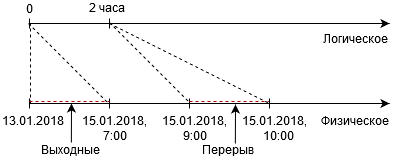
\includegraphics[width=\linewidth]{pics/scheduleAxes.png}
	\caption{Пример отображения оси логического на ось физического времени}
	\label{fig:axes}
	\centering
\end{figure}

\indent Как было сказано ранее, из-за того что рабочее время является дискретным, мы не имеем возможности просуммировать начальную дату и значение поданного логического времени.
Это ведет к тому, что необходимо синхронизировать логическое и физическое время,и это достигается путем последовательного периодического отображения конкретного логического времени на физическое (см. \ref{fig:axes}).
Это подразумевает под собой наличие двух массивов чисел или 'осей':

\begin{itemize}
	\item оси логического времени, которая начинается с нуля и единица которой соответствует одной секунде (необходимости в более точном отображении нет);
	\item оси физического времени, на которой может быть отложено любая дата физического времени, отсчет которой начинается 1 января 1970 года 00:00:00 (эпоха Unix).
\end{itemize}

Особенностью оси физического времени является наличие на ней 'выколотых' промежутков времени, в которые работа не ведется и операции не выполняются, следовательно, об этих промежутках системе необходимо знать, что подразумевает данную информацию как входные данные.
% Они передаются системе в виде структуры данных, которая далее будет называться 'конфигурацией модуля'.\\

\indent Входными данными для модуля являются:

\begin{itemize}
	\item дата с которой необходимо начинать отсчет;
	\item логическое время, которого необходимо достигнуть;
	\item конфигурация модуля.
\end{itemize}

\indent Дата является точкой на физической оси, на которую будет отображаться нуль логической. Представляет собой количество секунд, прошедшее с начала эпохи Unix.

\indent Логическое время~-~количество секунд, которое должно быть отложено на логической оси. В силу непрерывности физической оси, каждой логической точке сопоставляется отрезок на физической оси, сопоставляется пара чисел - границ данного отрезка.

\indent Конфигурация модуля~-~вспомогательные данные используемые для определения модулем какие промежутки необходимо пропускать в процессе работы.
Состоит из данных о рабочем графике занятого персонала (интервалы рабочего времени), шаблонном расписании на неделю (например, суббота, воскресенье - выходные, пятница - 'короткий' день, остальные - стандартные рабочие дни) и набор информации о датах, которые являются днями-исключениями и соответствующей информацией о графике работы в данные дни.
% \subsection{Результат работы}

% \subsection{Реализация}
\indent После запуска, модуль получает параметры и совершает проверку последних на корректность и непротиворечивость (например, если два дня имеют пересечения временных промежутков то они противоречивы, ведь ресурс не может работать одновременно в двух сменах) как в рамках смен одного так соседних дней.
Далее производится определение режима работы: прямой, обратный расчет или проверка времени:

\begin{itemize}
	\item прямой расчет - задается дата начала отсчета, логическое время и расчет ведется до нахождения даты окончания работ (см \ref{fig:straightCalc});
	\item обратный расчет - задается дата дедлайна, логическое время и расчет ведется до нахождения времени начала работ(см \ref{fig:reverceCalc});
	\item проверка времени - задается дата и логическое время равное нулю, что запускает оба предыдущих расчета пока не будет найдено первое ненулевое время в обоих направлениях от даты начала расчета(см \ref{fig:checkCalc}).
\end{itemize}

\begin{figure}[h]
	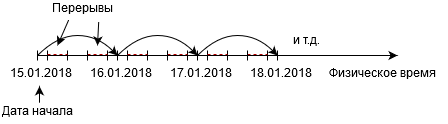
\includegraphics[width=\linewidth]{pics/scheduleStraightCalc.png}
	\caption{Схема прямого расчета}
	\label{fig:straightCalc}
	\centering
% \end{figure}
% \begin{figure}[h]
	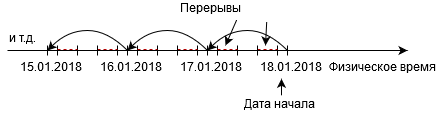
\includegraphics[width=\linewidth]{pics/scheduleReverceCalc.png}
	\caption{Схема обратного расчета}
	\label{fig:reverceCalc}
	\centering
% \end{figure}
% \begin{figure}[h]
	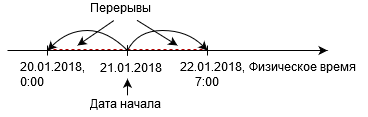
\includegraphics[width=\linewidth]{pics/scheduleCheckCalc.png}
	\caption{Схема проверки времени}
	\label{fig:checkCalc}
	\centering
\end{figure}

\indent Выбрав режим работы сбрасывается счетчик текущего логического времени до нуля и счетчик текущего физического времени до стартовой даты. Затем итеративно, пока текущее логическое время не превысит необходимое производится поиск следующей даты.
Алгоритмически, поиск даты работает следующим образом:

\begin{enumerate}
	\item[\mylabel{itm:point1}{1})] определяются интервалы рабочих смен относящихся к текущему дню:
	      \begin{enumerate}
		      \item[а)] при отсутствии таковых, к текущей дате прибавляется один день и затем возврат к п.\ref{itm:point1}.
	      \end{enumerate}
	\item[2)] отсортированные в порядке возрастания интервалы последовательно перебираются и их длительности прибавляются к текущему логическому и физическому времёнам:
	      \begin{enumerate}
		      \item[а)] при превышении текущим логическим временем необходимого, переход к п.\ref{itm:point3};
		      \item[б)] если все интервалы были просуммированы, но необходимое логическое время не превышено - переход к п.\ref{itm:point1};
	      \end{enumerate}
	\item[\mylabel{itm:point3}{3})] разность текущего и необходимого логического времён вычитается из физического времени, при этом сохраняя данное значение как левую (правую при обратном расчете) границу и продолжается расчет для выявления правой (левой) границы промежутка.
\end{enumerate}

\begin{figure}[h]
	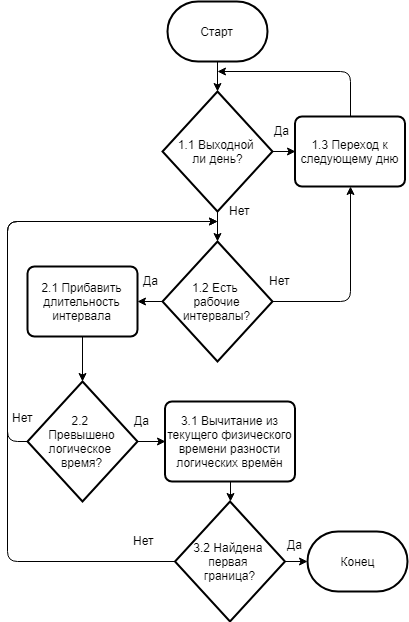
\includegraphics[width=\linewidth]{pics/scheduleSchema.png}
	\caption{Блок-схема модуля}
	\label{fig:schema}
	\centering
\end{figure}

\indent Определение интервалов рабочего времени происходит взятием даты из текущего физического времени, после чего начинается определение принадлежности данной даты к перенесенным датам после чего есть два варианта развития ситуации:

\begin{itemize}
	\item дата является перенесенным днем и модуль получает информацию о расписании которое нужно применить;
	\item дата не является перенесенным днем и получение информации происходит исходя из того, каким днем недели является данная дата.
\end{itemize}

\begin{figure}[h]
	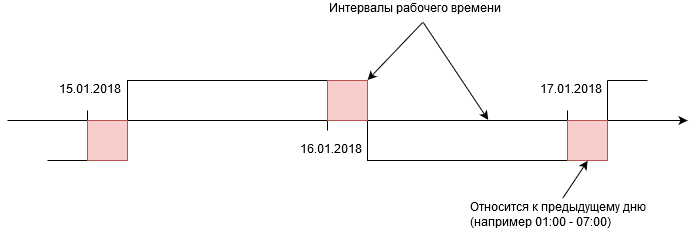
\includegraphics[width=\linewidth]{pics/scheduleIntervals.png}
	\caption{Смещение интервалов рабочего времени относительно рабочего дня}
	\label{fig:intervals}
	\centering
\end{figure}

\indent Так как на реальных производственных площадках нередко случается так, что рабочие интервалы, принадлежащие к рабочему дню и сам рабочий день смещены относительно друг друга (см. \ref{fig:intervals}).
При этом возникают трудности с определением интервалов рабочего времени в связи с тем, что для определения используется количество секунд с начала эпохи Unix и до нуля часов нуля минут и нуля секунд нужной даты, по которому, используя инструментарий языка, каким днем недели является нужная дата и, соответственно, задать для нее шаблон рабочего времени.
И если эти трудности практически не влияют на прямой расчет, то с обратным все немного сложнее.
Так как одном дне 86400 секунд и, если рассматривать границу двух дней (см. \ref{fig:time}), то 86400 секунда предыдущего дня будет равна или тем же что и нулевая секунда нового дня.
Можно сказать, что 86400 - левый предел, а 0 - правый предел в данной точке (особенно если изображать в виде окружности).
Но, в связи с тем, что данная недетерминированность присутствует лишь при рассмотрении человеком данной ситуации, а система может распознавать диапазон от 0 до 86399 секунд, то для определения интервалов рабочего графика (при обратном расчете) используется именно величина в 86399 секунд, при условии, что данное допущение не влияет на расчет, как последняя секунда текущего дня.

\begin{figure}[h]
	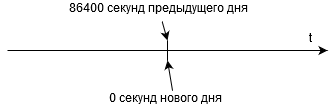
\includegraphics[width=\linewidth]{pics/scheduleTime.png}
	\caption{Граница двух дней}
	\label{fig:time}
	\centering
\end{figure}

\indent Возвращаясь к пункту \ref{itm:point3} алгоритма, при нахождении нужного времени, работа модуля не прекращается, а ведется до момента нахождения второй границы промежутка, на который отображается необходимое логической время.

\indent Как было сказано ранее - физическое время непрерывно, а следовательно когда производится отображение на него логического времени, в результате должен получиться промежуток (см. \ref{fig:axes}), который и характеризуют две границы.
Эта пара чисел, характеризующие начало и конец отрезка которые отображаются на логическую ось в точке, значение которой равно входному логическому времени и являются выходными данными данного модуля.

\begin{figure}[ht]
	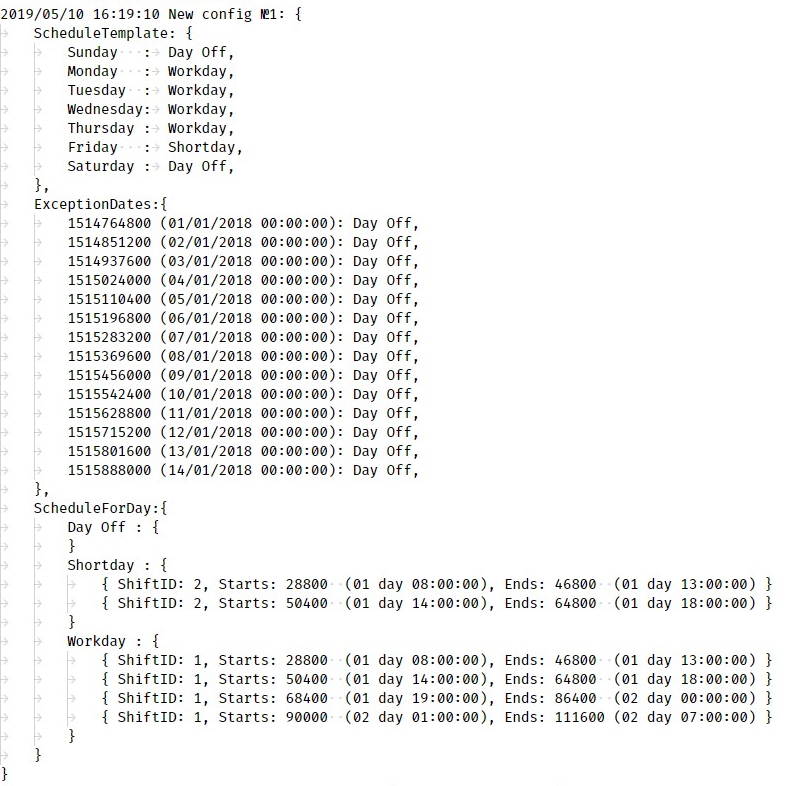
\includegraphics[scale=0.7]{pics/scheduleConfigExample.png}
	\caption{Пример конфигурации модуля}
	\label{fig:config}
	\centering
\end{figure}

\indent В результате работы над модулем были написаны тесты и проведено тестирование, результаты одного из которых можно увидеть на изображениях \ref{fig:config} и \ref{fig:eval1}.
На \ref{fig:config} изображена конфигурация модуля, которая показывает как производится совмещение логического и физического дня, обработка перенесенных дней.
На \ref{fig:eval1}, перед расчетом нового отображения, можно отметить, что при использовании той же конфигурации не производится ее повторный вывод в лог, что позволяет сократить его длину, а следовательно улучшить читаемость.
Рисунок \ref{fig:eval1} показывает итеративный процесс как результат прибавления каждого нового интервала к текущему времени.

\begin{figure}[ht]
	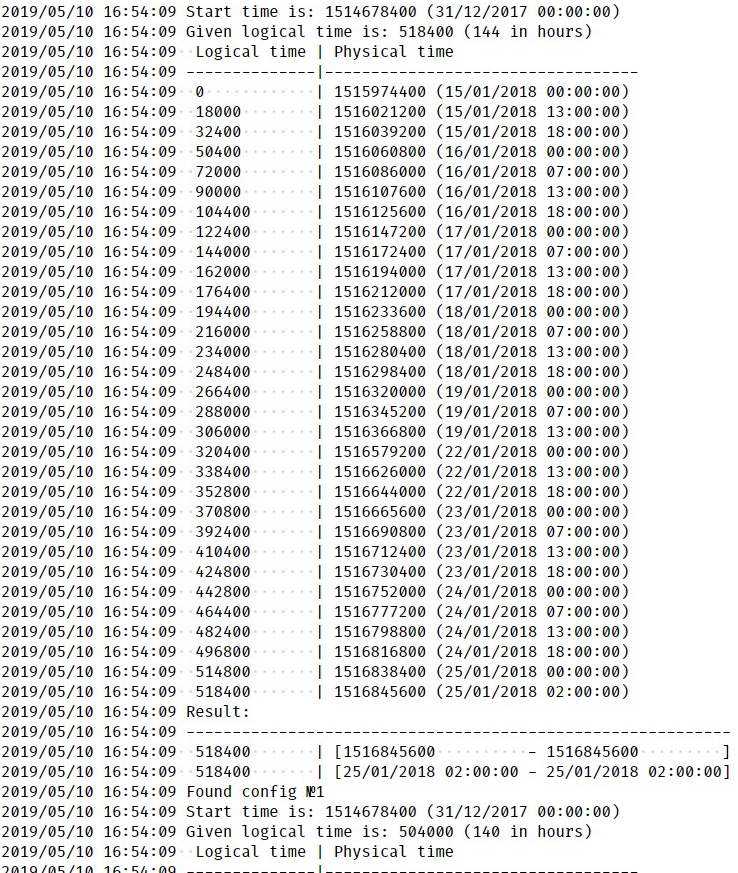
\includegraphics[scale=0.6]{pics/scheduleEvalExample.png}
	\caption{Пример прямого расчета модулем}
	\label{fig:eval1}
	\centering
\end{figure}


\begin{figure}[ht]
	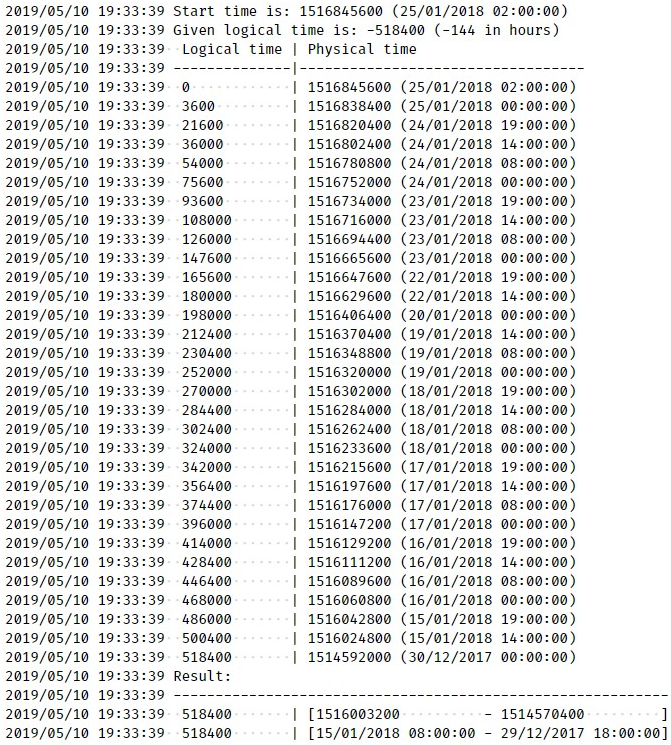
\includegraphics[scale=0.6]{pics/scheduleRevertEvalExample.png}
	\caption{Пример обратного расчета модулем}
	\label{fig:revEval}
	\centering
\end{figure}

\indent Также были проведены тесты обратного расчета и проверки времени, результаты которых можно видеть на изображениях \ref{fig:revEval} и \ref{fig:checkEval}.
Пояснение к проверке даты: тут используется конфигурация, когда 2 января является выходным, проверка которой и производится, что позволяет продемонстрировать работу данного решения.


\begin{figure}[ht]
	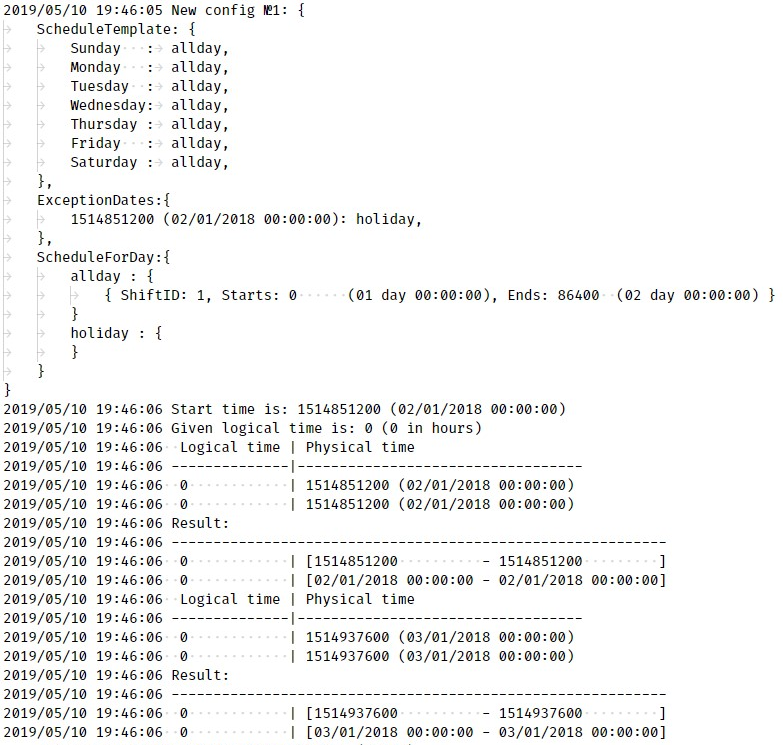
\includegraphics[scale=0.6]{pics/scheduleCheckDateEval.png}
	\caption{Пример проверки модулем времени}
	\label{fig:checkEval}
	\centering
\end{figure}

% \todo[inline]{пояснение трудностей}

% При обратном расчете, если использовать ту же последовательность действий, то получится, что система будет выбирать шаблон 
% \todo[inline]{Так как расчет расписания — это итеративный процесс, то в рамках разработки было выделено понятие временной линии (прямой) – это «линия» на которой для каждой точки, которая является абстрактной величиной времени выполнения операции, сопоставляются две даты соответствующие данной абстрактной величине времени с учетом расписания. Первая дата является концом данной операции, вторая – началом следующей. Данное разделение было использовано, потому как все время что между ними также относится к данной точке, а значит каждой точке, из-за непрерывности времени, соответствует бесчисленное множество точек на временной прямой, что может быть лишь ограничено двумя границами – временем начала и конца данного отрезка.}

% при попытке получения интервалов для текущей дата, которая, например, исходя из рисунка \ref{fig:intevals}, 17.01.2018, получаются интервалы для 17.01.2018, а не для 16.01.2018, хотя, как можно предположить, 00:00 17.01.2018 и 24:00 16.01.2018 равны

\chapter{Организация консистентного хранилища данных}

\section*{Выбор хранилища данных}

\indent Система планирования производства, как и практически любая система получающая и обрабатывающая данные, нуждается в хранилище данных - базе данных.
Хранилище данных может быть разделено на две составляющие:
\begin{itemize}
	\item хранилище временных данных;
	\item хранилище постоянных данных.
\end{itemize}

\indent Под временными данными подразумеваются данные, которые получаются в процессе работы системы (например оперативные и объемно-календарные планы) и, при необходимости, могут быть рассчитаны заново, хоть и с некоторыми затратами (время, вычислительные мощности), при условии отсутствия хранилища данных.
В данной работе этот вид данных и хранилище для них не рассматривается.\\
\indent С другой стороны постоянные данные - данные, которые задаются пользователем (в данном случае организацией) и потеря которых в лучшем случае приведет к необходимости заново добавлять их в систему, а в худшем - приведет к утрате этих данных.
В любом случае потеря постоянных данных ведет к нарушениям в работе системы, что ведет к необходимости организации консистентного хранилища данных.\\
\indent Консистентность - требование к данным, получаемым из базы данных, которое заключается в том, что последние должны быть целостны и непротиворечивы.
Под целостностью данных подразумевается соответствие имеющейся в базе данных информации её внутренней логике, структуре и явно заданным правилам.
Любое правило, направленное на ограничение возможного состояния базы данных называют ограничением целостности.
Помимо целостных, данные должны также быть непротиворечивыми, что означает, что в базе данных нет логического противоречия, то есть некоторого утверждения и его отрицания.
Со стороны систем управления базами данных (совокупность программных и лингвистических средств общего или специального назначения, обеспечивающих управление созданием и использованием баз данных) свойство консистентности выполняется на уровне транзакций (одним из требований к которой и является консистентность): если одна из команд транзакции не прошла проверку ограничений целостности, то вся транзакция откатывается, то есть база данных возвращается в состояние, в котором была начата транзакция.\\
\indent Транзакция - группа последовательных операций с базой данных, которая представляет собой логическую единицу работы с данными.
Транзакция может либо быть целиком и успешно независимо от идущих параллельно транзакций и соблюдая все ограничения целостности, либо не быть выполненной вообще, что в таком случае не должно оказать на систему никакого влияния.\\
\indent В соответствии с требованиями описанными выше, можно сделать вывод о необходимости использования реляционной базы данных, одним из преимуществ которой является соответствие требованиям ACID (Atomicity, Consistency, Isolation, Durability - атомарность, консистентность, которая и интересует в первую очередь, изолированность, долговечность).

\section*{Структура базы данных}

\indent Из предыдущей главы видно, что в постоянной базе данных необходимо хранить информацию по которой будет производиться расчет объемно-календарного и оперативного планов.
Для этого необходимо хранить:

\begin{itemize}
	\item данные о заказах;
	\item данные о типах продукции;
	\item данные о продукции, которая относится к каждому заказу;
	\item данные о самой последовательности операций и самих операциях для каждого типа продукции;
	\item данные о каждой модели ресурсов;
	\item данные о связях между моделью ресурса и операциями.
\end{itemize}

\begin{figure}[ht]	
	\centering	
	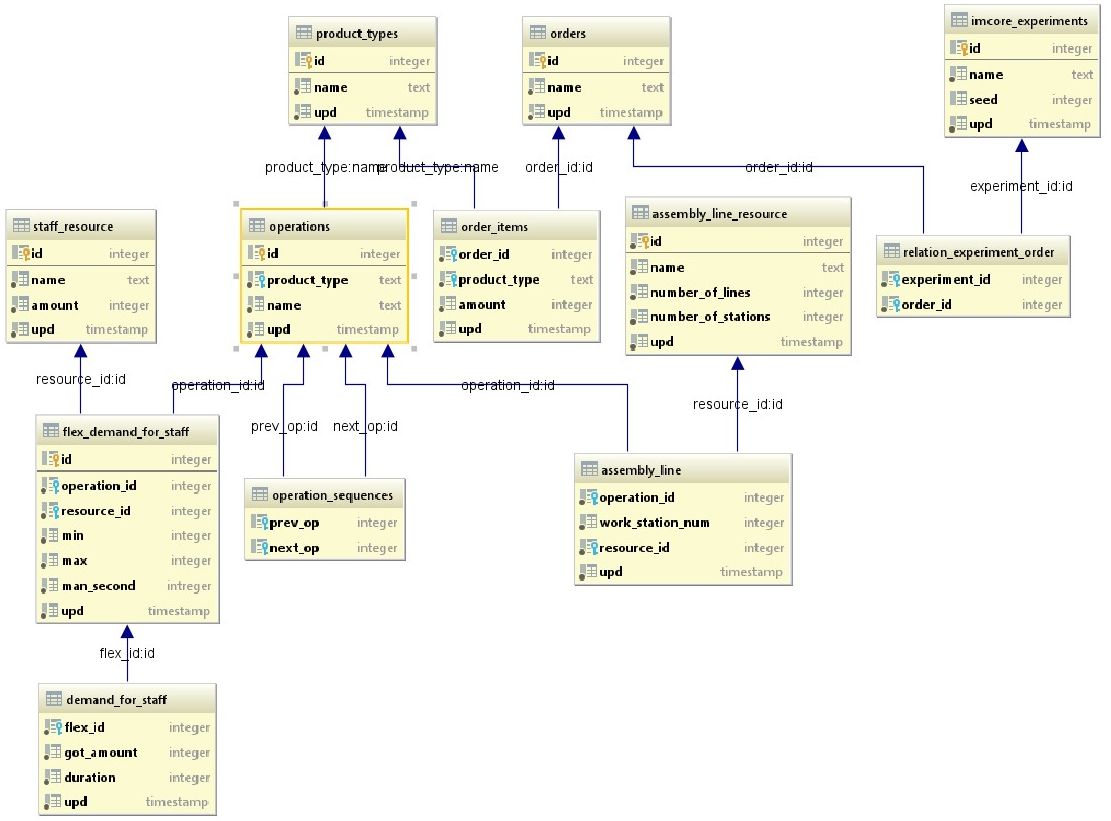
\includegraphics[width=\linewidth]{pics/databaseSchema.png}
	\caption{Схема базы данных}
	\label{fig:dbSchema}
\end{figure}

\indent Помимо этого, нужно учитывать, что кроме простого хранения данных, необходимо соблюдать 'версионность', ввиду того, что карта технологического процесса может меняться во времени, а значит и в базе данных, требуется следить за тем, чтобы в любой момент времени было возможно использовать любую из версий данной карты, иначе новый расчет оперативного плана (при условии, что другие данные остались неизменными) приведет к созданию новой версии плана, а, следовательно, предыдущую версию восстановить будет либо очень сложно, либо, в худшем случае - невозможно.\\
\indent Для достижения данной цели, в определенных таблицах было введено дополнительное поле - временная отметка обновления - 'upd'.
С помощью этой метки можно как получить последние данные из базы, просто максимизируя метку 'upd', так и получить данные на определенный момент времени ограничивая эту метку необходимым временем.

\section*{Обоснование/Доказательство}
\indent Теория реляционных баз данных оперирует понятиями отношения (relation), от которого и пошло само название теории и баз данных основанных на ней, атрибута, домена, кортежа.

\begin{figure}[ht]
	\centering
	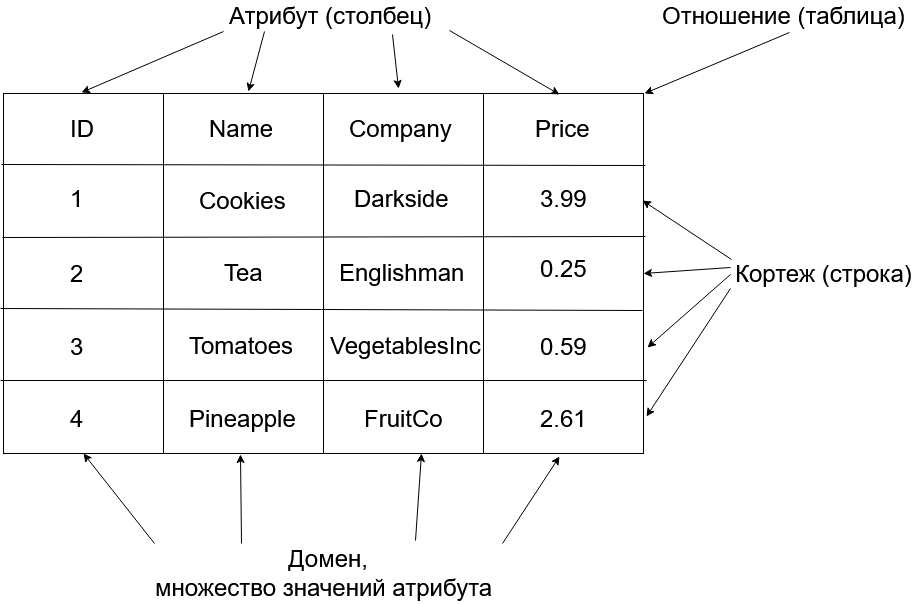
\includegraphics[width=\linewidth]{pics/databaseExample.png}
	\caption{Понятия реляционной базы данных}
	\label{fig:dbExample}
\end{figure}

\indent Атрибут - именованный столбец отношения.
В пределах одного атрибута все значения должны быть одного типа данных, то есть принадлежать одному домену.\\
\indent Домен - тип данных, множество всех допустимых значений атрибута.\\
\indent Кортеж - упорядоченный набор из N элементов, где N - это число атрибутов отношения.
По-другому можно сказать, что кортеж это строка или запись таблицы.\\
\indent Отношение - множество упорядоченных N-кортежей.
Другими словами отношение - это двумерная (плоская) таблица, состоящая из столбцов и строк - атрибутов и кортежей.(см. \ref{fig:dbExample})\\

\todo[inline]{математическое обоснование}
\todo[inline]{полностью переписать, исключить ACID}

\section{Теорема}
\begin{theorem}
	\label{th:th1}
	В любой момент времени можно восстановить необходимую версию карты технологического процесса, при условии того, что известно её имя и значение точки версионирования, которое не меньше заданного в базе данных для искомой карты и не больше и не равно следующей точки версионирования.
\end{theorem}

\begin{proof}[Доказательство]
	Используя метод доказательства от противного, предположим, что нельзя восстановить необходимую версию карты технологического процесса, при условии того, что известно её имя и значение точки версионирования, которое не меньше заданного в базе данных для искомой карты и не больше и не равно следующей точки версионирования из чего следует утверждение \ref{st:st1}.
	\begin{state}
		\label{st:st1}
		Нельзя создать такой запрос, который, для всех имён карт технологического процесса из домена 'name' отношения 'product\_types' и любой заданной точки версионирования построит нужную карту.
	\end{state}

	\begin{figure}[ht]
		\centering
		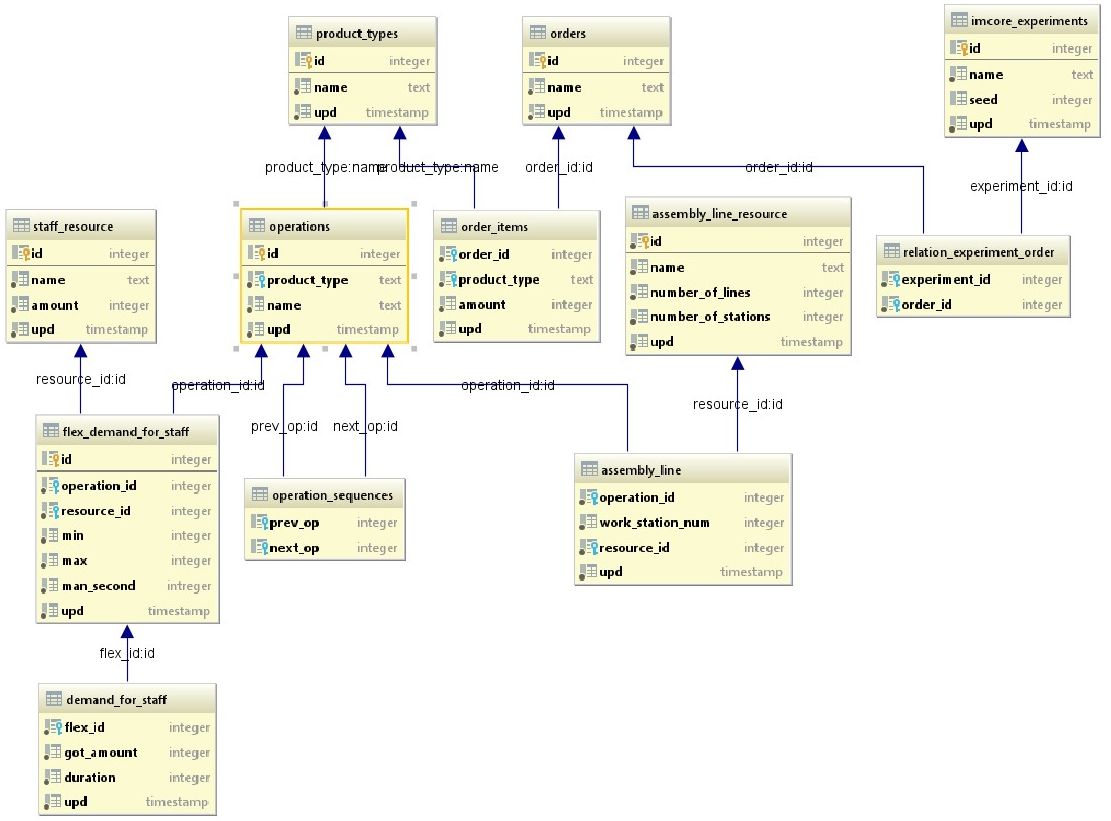
\includegraphics[width=\linewidth]{pics/databaseSchema.png}
		\caption{Схема базы данных}
		\label{fig:dbschema}
	\end{figure}

	\indent Используя схему БД, представленную на рисунке \ref{fig:dbschema}, постараемся доказать обратную теорему.\\
	\indent Введем сокращения названий отношений:

	\begin{itemize}
		\item $product\_types \Rightarrow pr$;
		\item $operations \Rightarrow ops$;
		\item $operation\_sequences \Rightarrow seq$.
	\end{itemize}

	\indent Предположим, есть переменная, принадлежащая домену 'name'\ отношения 'product\_types'\ $pr\_name \in pr.name$ и переменная $pr\_upd \in \mathbb{Z}$, заданные пользователем, тогда запишем запросы:
	\begin{equation}
		\label{eq:upd}
		pr\_upd' \leftarrow \pi_{pr.upd}(\sigma_{pr.name\ =\ pr\_name\ AND\ pr.upd\ \leq\ pr\_upd}\ pr)
	\end{equation}
	\begin{equation}
		\label{eq:ops}
		ops' \leftarrow \pi_{ops.id,\ pr.name,\ ops.upd}(pr \bowtie_{pr.name = ops.product\_type} ops)
	\end{equation}
	\begin{equation}
		\label{eq:seq}
		seq' \leftarrow \pi_{ops'.upd,\ ops'.name,\ seq.prev\_op,\ seq.next\_op}(ops' \bowtie_{ops'.id = seq.prev\_op} seq)
	\end{equation}
	\begin{equation}
		\label{eq:chart}
		chart \leftarrow \pi_{prev\_op,\ next\_op} (\sigma_{seq'.name\ =\ pr\_name\ AND\ seq'.upd\ =\ pr\_upd'\ } seq')
	\end{equation}

	\indent Проведем анализ полученных запросов:
	\begin{enumerate}
		\item[1)] в выражении \ref{eq:upd} производится извлечение значения ближайшей (и не большей чем заданная пользователем) точки версионирования;
		\item[2)] затем в выражении \ref{eq:ops} производится объединение отношений 'product\_types' и 'operations' по атрибуту имени карты технологического процесса, в результате получаем все операции всех карт технологического процесса всех точек версионирования;
		\item[3)] после этого в выражении \ref{eq:seq} объединяются отношение \ref{eq:ops} и 'operation\_sequences', что дает все последовательности операций для всех карт технологического процесса всех точек версионирования;
		\item[4)] и в \ref{eq:chart} производится выборка последовательностей из \ref{eq:seq} по имени карты процесса и полученной в выражении \ref{eq:upd} точки версионирования.
	\end{enumerate}

	\indent Так как карта технологического процесса записывается полностью и с одним значением точки версионирования для всех элементов, то мы получаем выборку карты, с заданным именем, которое существует в домене 'name' отношения 'product\_types' и с значением точки версионирования, которая существует в домене 'upd' того же отношения и, соответственно, является искомой картой.
	Создание такого запроса опровергает утверждение \ref{st:st1}, а следовательно доказывает теорему \ref{th:th1}.
\end{proof}
\section*{Заключение}
\addcontentsline{toc}{chapter}{Заключение}
В рамках данной работы были рассмотрены, разработаны и протестированы компоненты системы планирования производства, а также организованно хранилище данных, работа которого была формально верифицирована.

По итогу выполнения работы были достигнуты следующие результаты:
\begin{itemize}
	\item произведен анализ логического и физического времени;
	\item синтезирован, реализован и протестирован алгоритм отображения логического времени на физическое;
	\item проанализирована сборочная линия, её функции и ограничения, накладываемые на перемещение продукции;
	\item синтезирована, реализована и протестирована модель сборочной линии для подсистемы имитационного моделирования СПП;
	\item проанализированы данные предприятия, которые необходимо хранить в базе данных;
	\item синтезирована и обоснована структура базы данных.
\end{itemize}

\indent Разработанные модули в настоящий момент интегрированы в СПП с соответствующими интеграционными тестами.\\
\indent Структура базы данных была реализована и используется для хранения и извлечения тестовых данных\todo{обезличенных, ссылка на Диаконт без упоминания?}, что используется для тестирования ядра имитационного моделирования. 
Также были реализованны введенные в процессе обоснования структуры базы данных операторы и выражения, что упростило работу с версионированными отношениями.

% В данной работе был проведен анализ и разработка компонент системы планирования производства, являющуюся частью интегрируемого программного комплекса интеллектуальной системы управления предприятием, и, впоследствии, были внедрены в данную систему.

% \indent В результате был разработан и протестирован алгоритм отображения логического времени на физическое, позволяющий:
% \begin{itemize}
% 	\item производить гибкую настройку своей работы путем изменения конфигурации рабочего календаря;
% 	\item производить как прямой так и обратный расчет;
% 	\item отслеживать корректность работы путем ручного (при помощи логов) и автоматизированного тестирования.
% \end{itemize}
\todo[inline]{Написать и исправить}


% КОНЕЦ ТЕКСТА
%%%%%%%%%%%%%%%%%%%%%%%%%%%%%%%%%%%%%%%%%%

\backmatter{} %% Здесь заканчивается нумерованная часть документа и начинаются ссылки и
\bibliography{bib/bibl}{}
\bibliographystyle{plain}

\end{document}
